\chapter{}
\section{8-by-8 Grid World}
This figure shows an example initial data set, $D^{(0)}$ used in line $3$ of Algorithm \ref{alg:single_agent_single_update}.


\begin{figure}[htb]
	\begin{center}
		\fbox{
			\begin{minipage}{0.7\textwidth}
				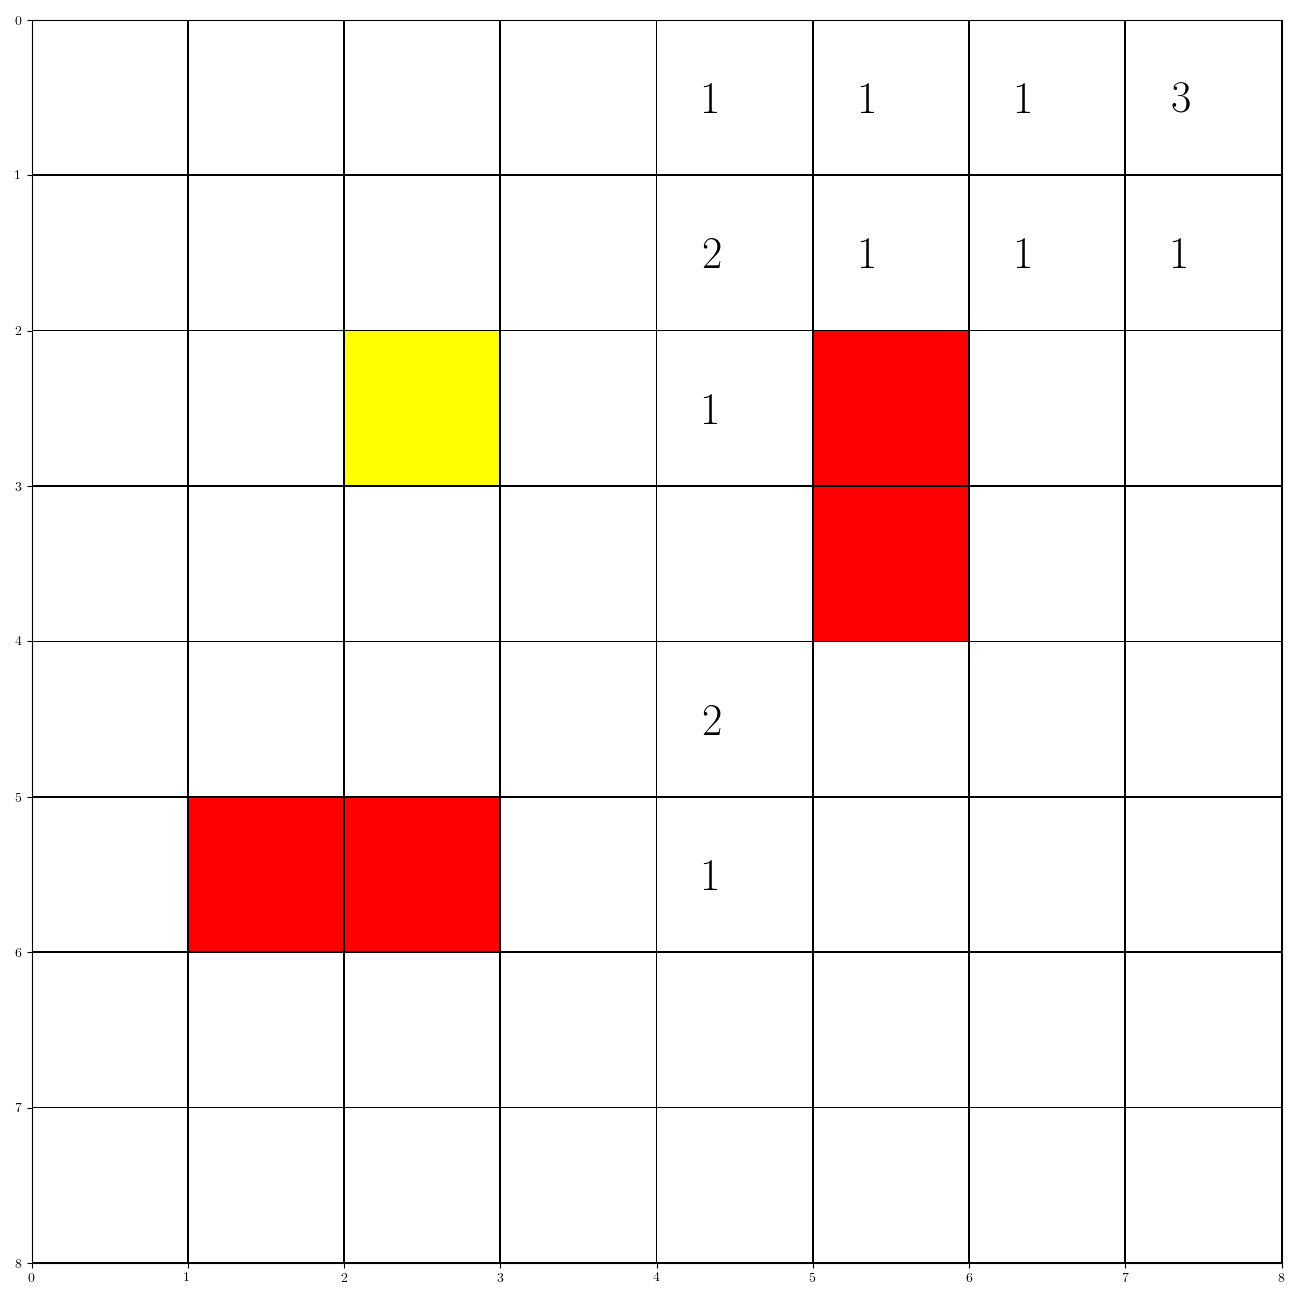
\includegraphics[width=\textwidth]{8x8_sparse_demo}
				\caption{8-by-8 grid world for a single agent.}
				\label{fig:8-by-8_grid_world}
			\end{minipage}
		}
	\end{center}
\end{figure}

\section{32-by-32 Grid World}\label{sec:32by32grid}

\begin{figure}[H]
	\begin{center}
		\fbox{
			\begin{minipage}{1\textwidth}
				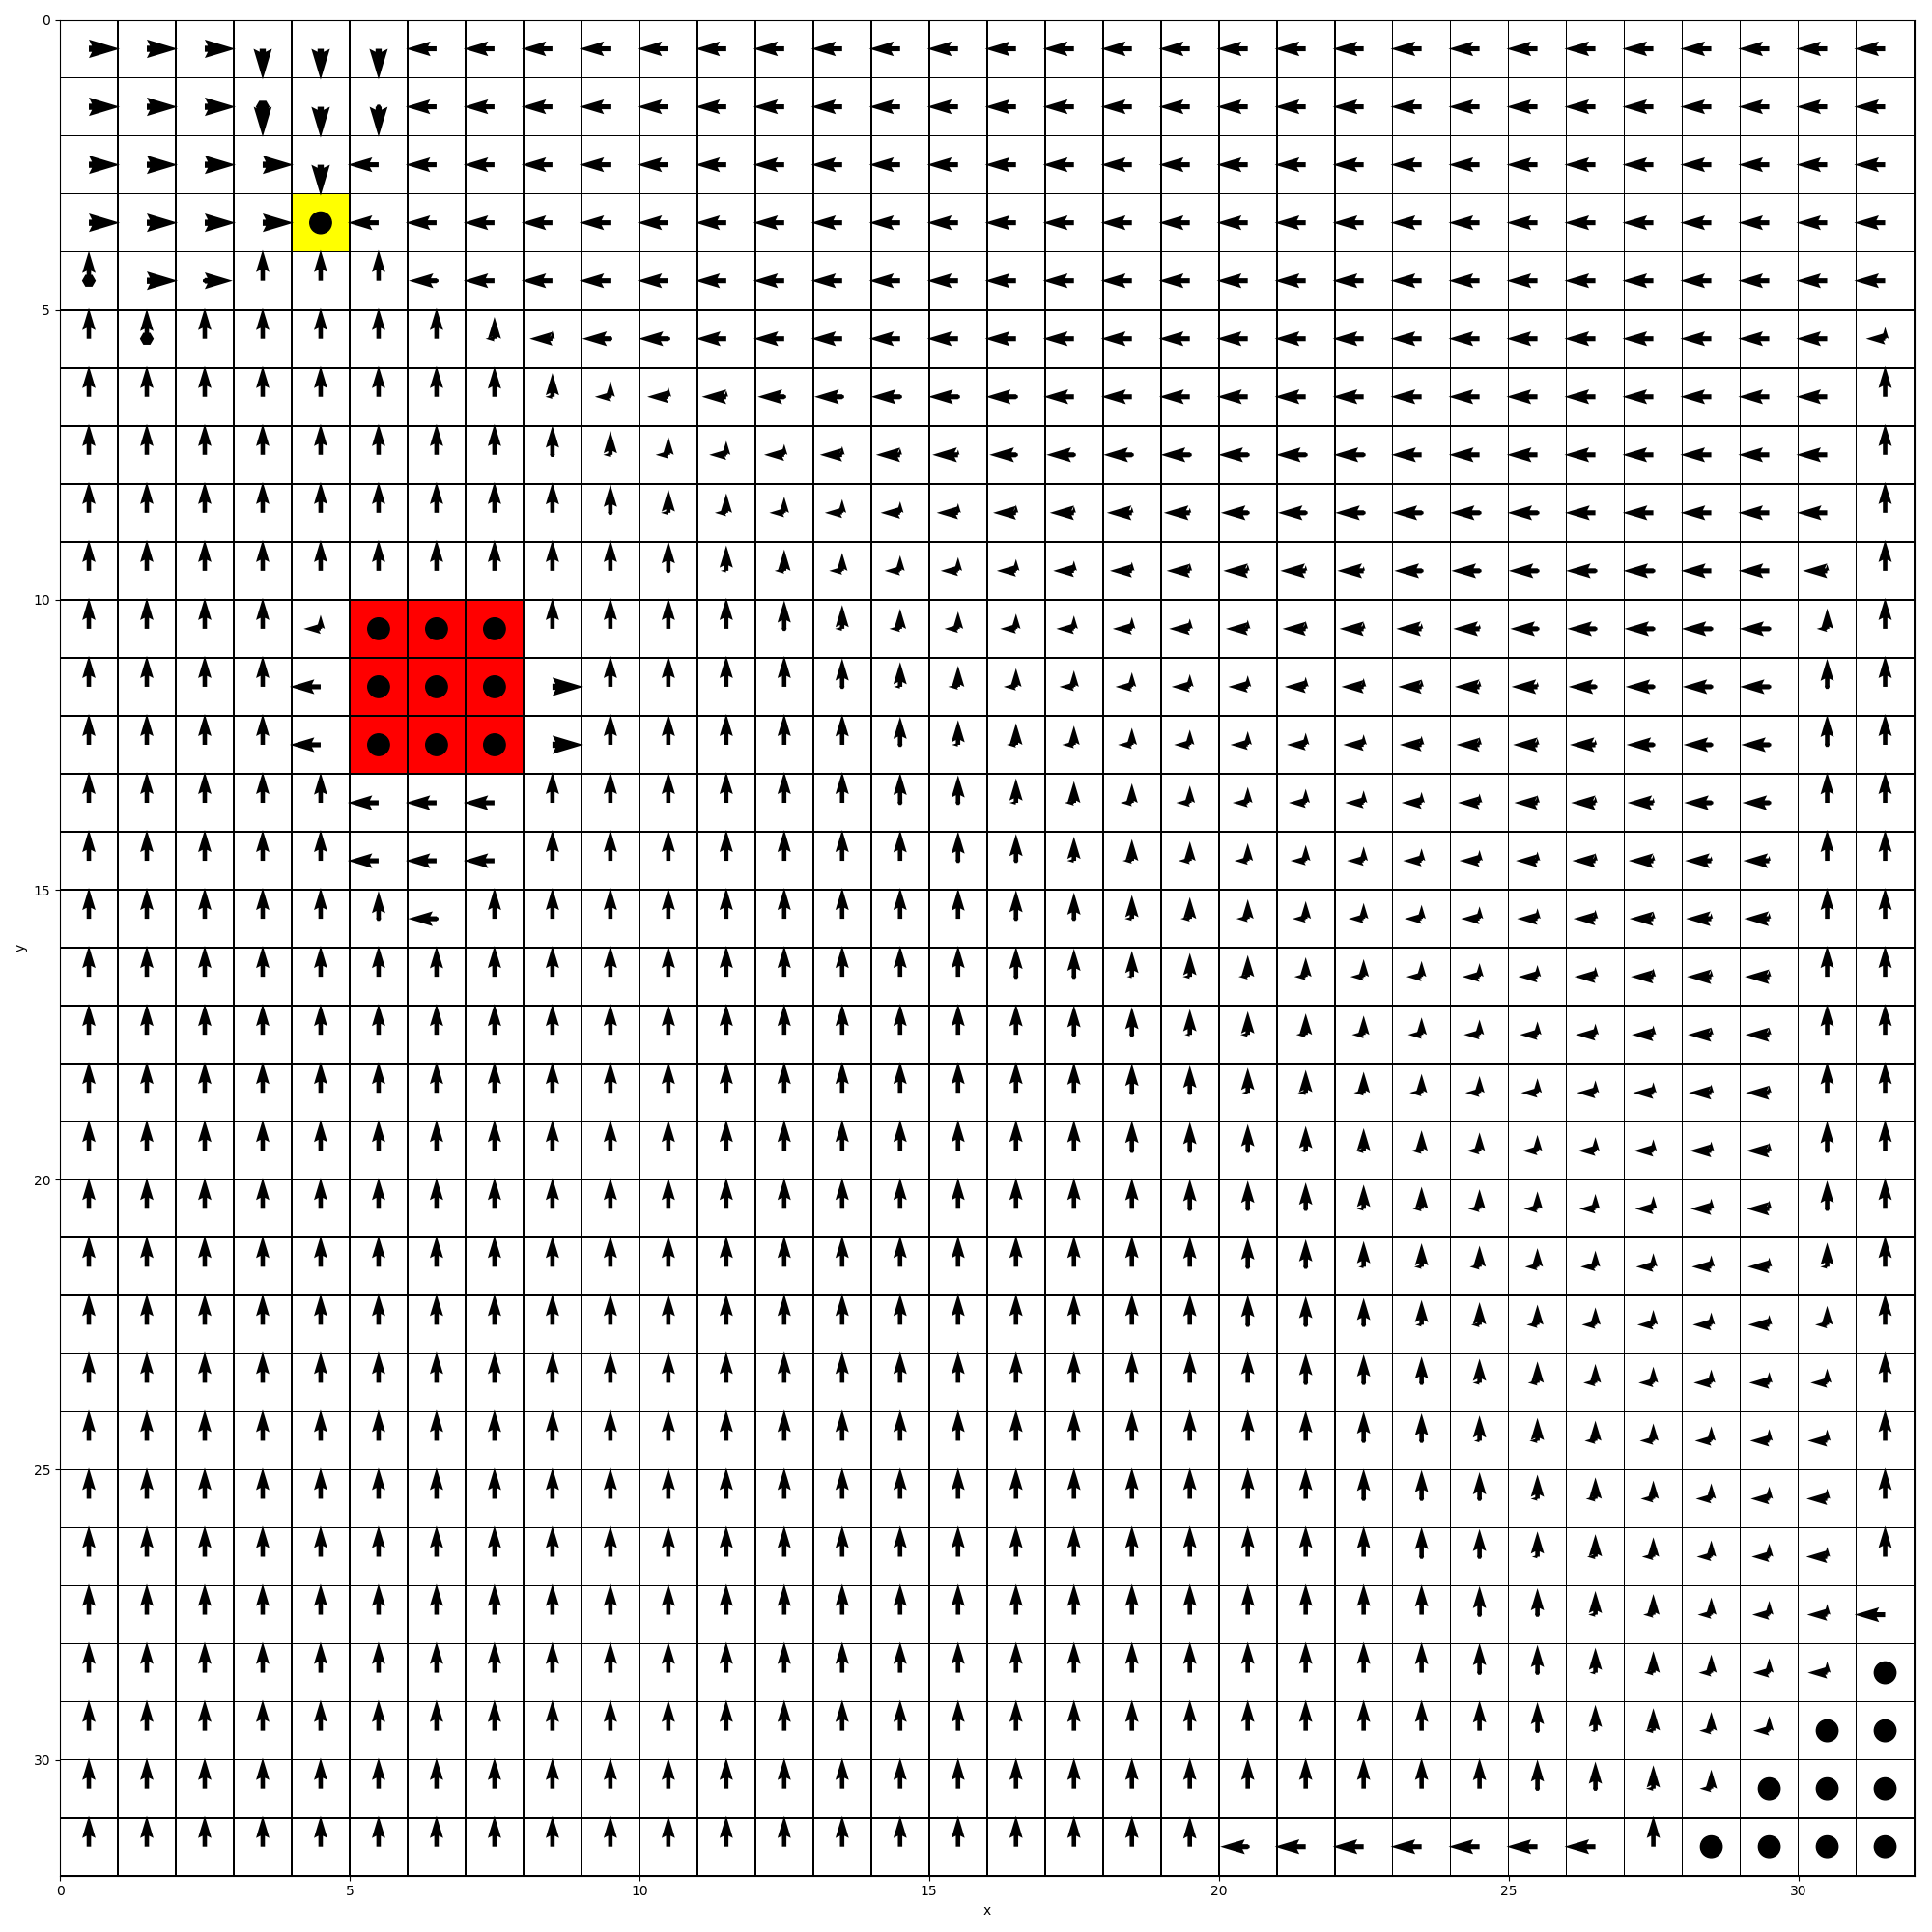
\includegraphics[width=\textwidth]{large_grid_true_policy}
				\caption{True policy of \agent{2} in a single agent environment. Grid size is 32-by-32. Arrow sizes are proportional to probability of taking the action in each direction. Dots represent the stay-action.}
				\label{fig:large_grid_true_policy}
			\end{minipage}
		}
	\end{center}
\end{figure}


\begin{figure}[H]
	\begin{center}
		\fbox{
			\begin{minipage}{1\textwidth}
				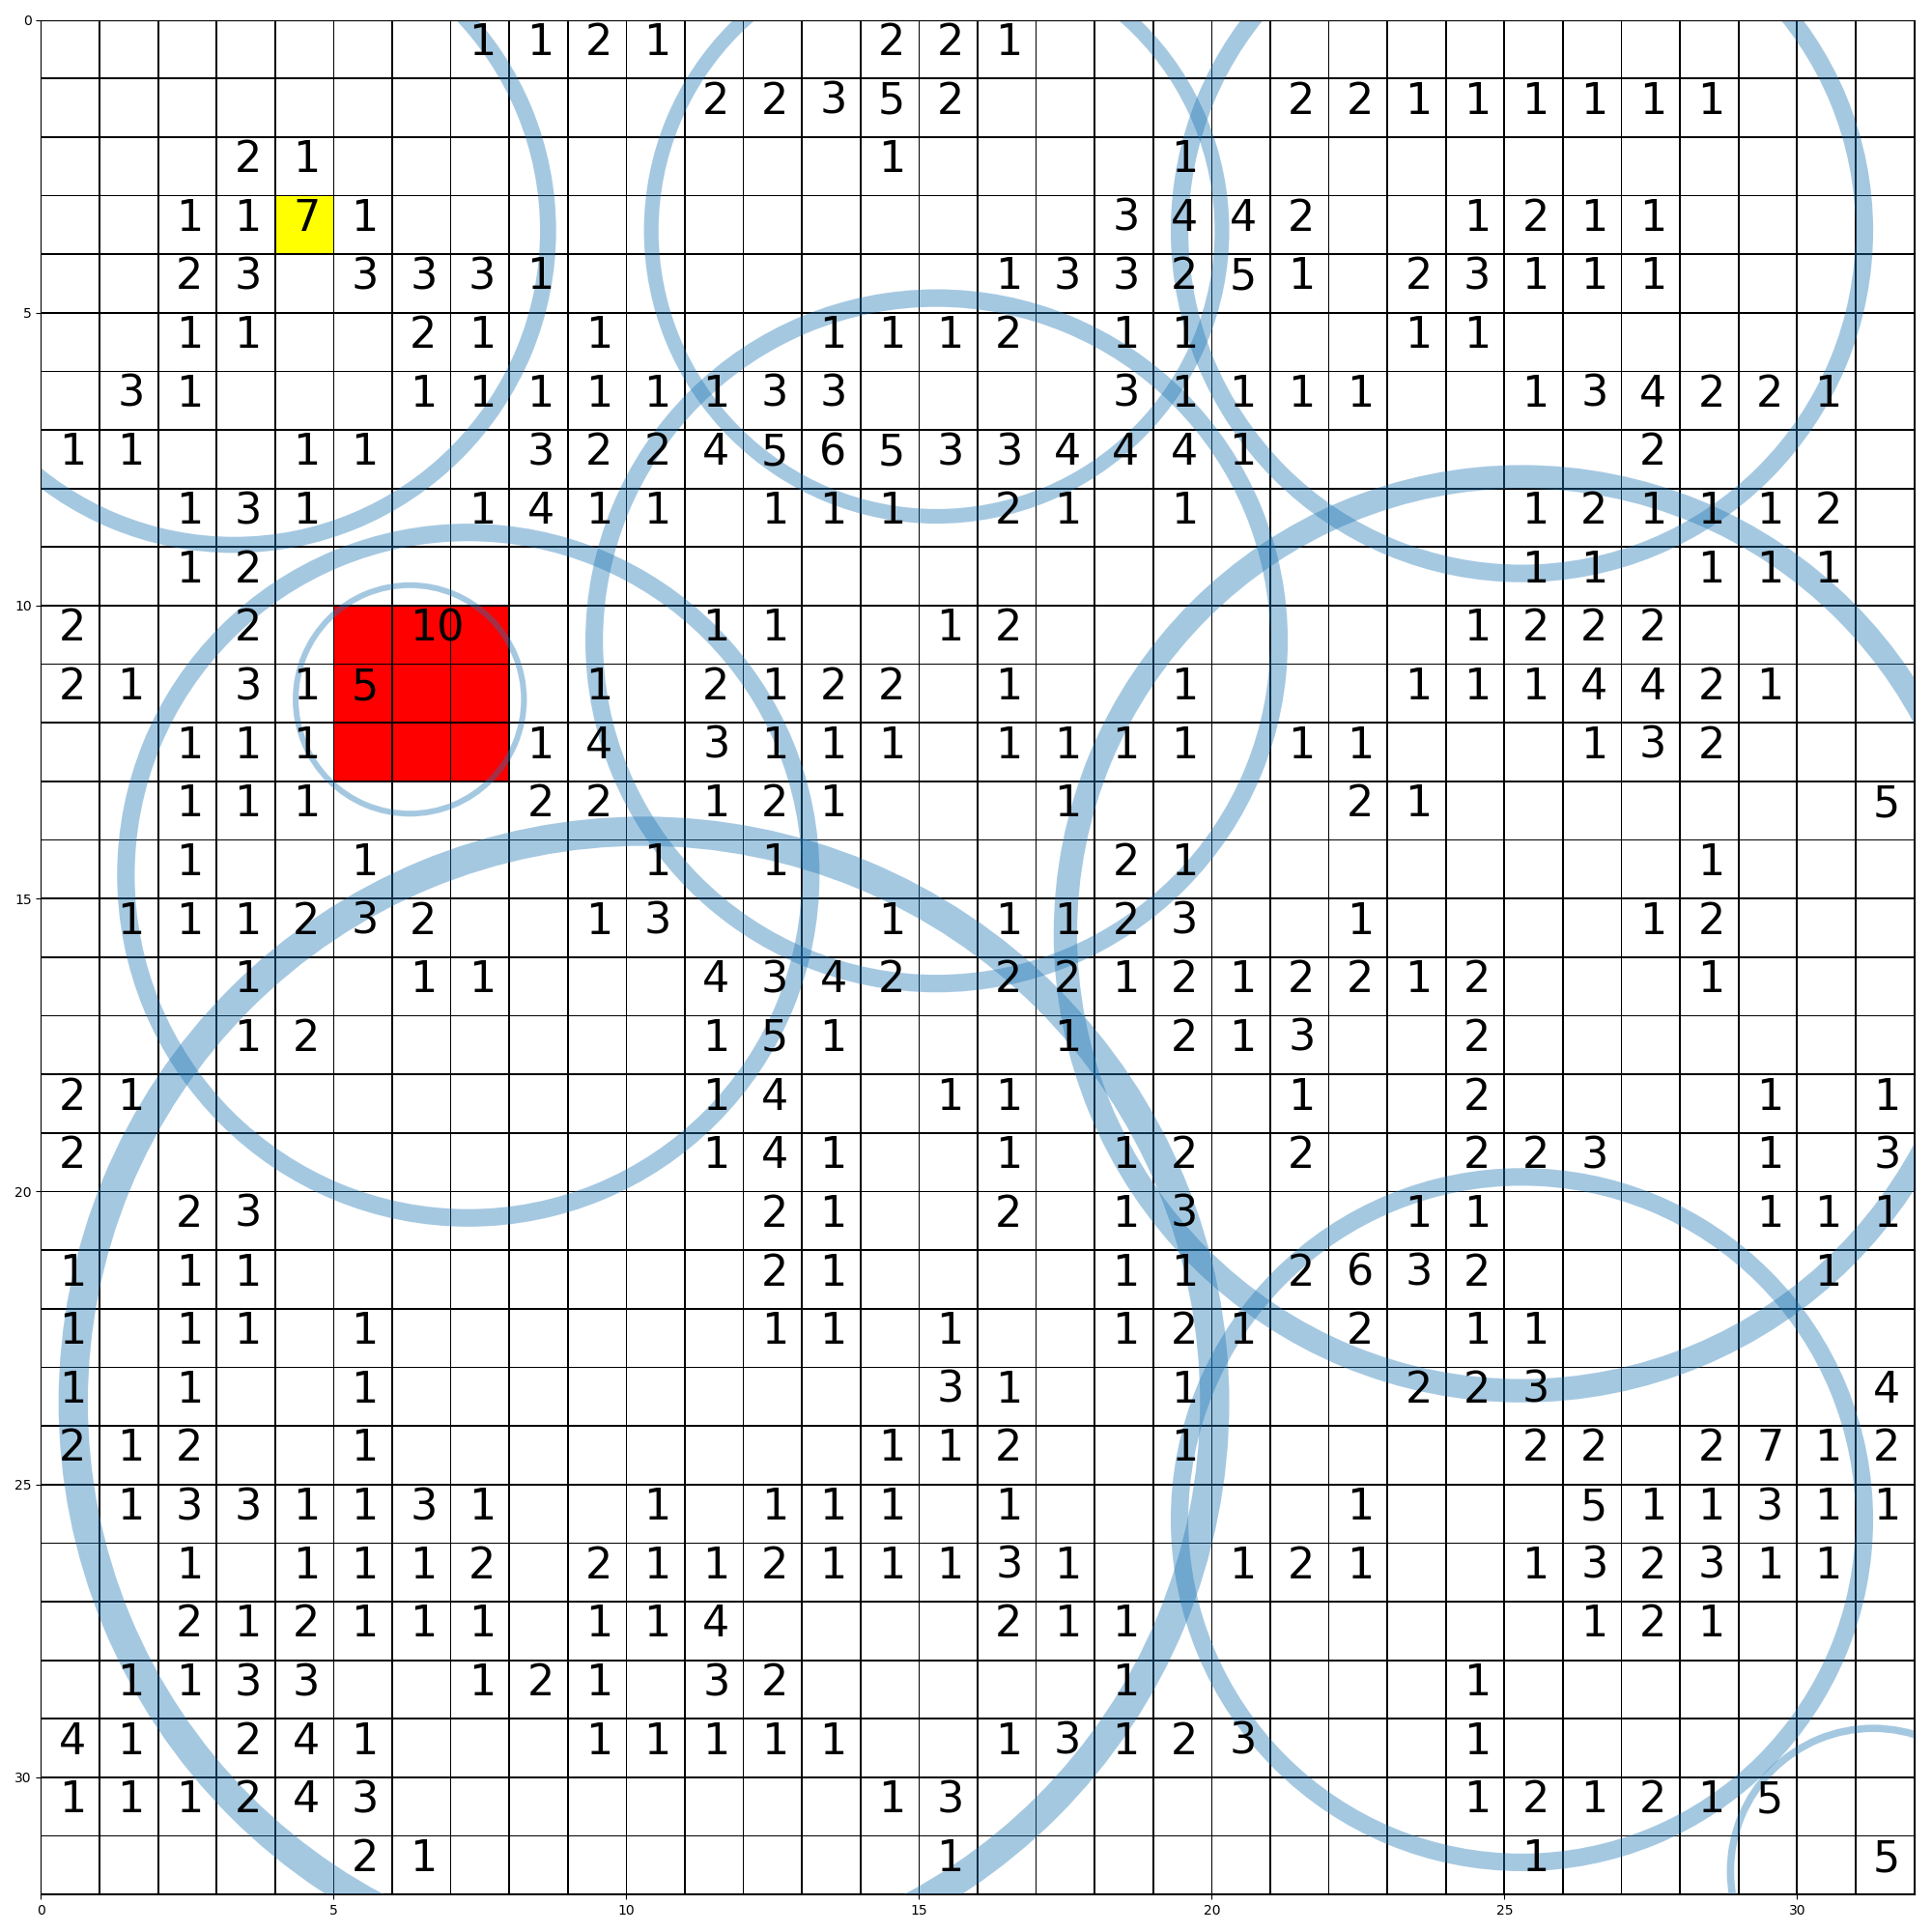
\includegraphics[width=\textwidth]{large_grid_visit_count}
				\caption{Visitation count given 150 trajectories with 5 time steps using the true policy of \agent{2} (Fig. \ref{fig:large_grid_true_policy}) in a single agent environment. Grid size is 32-by-32. Blue circles represent the standard deviation of kernels used.}
				\label{fig:large_grid_visit_count}
			\end{minipage}
		}
	\end{center}
\end{figure}


\begin{figure}[H]
	\begin{center}
		\fbox{
			\begin{minipage}{1\textwidth}
				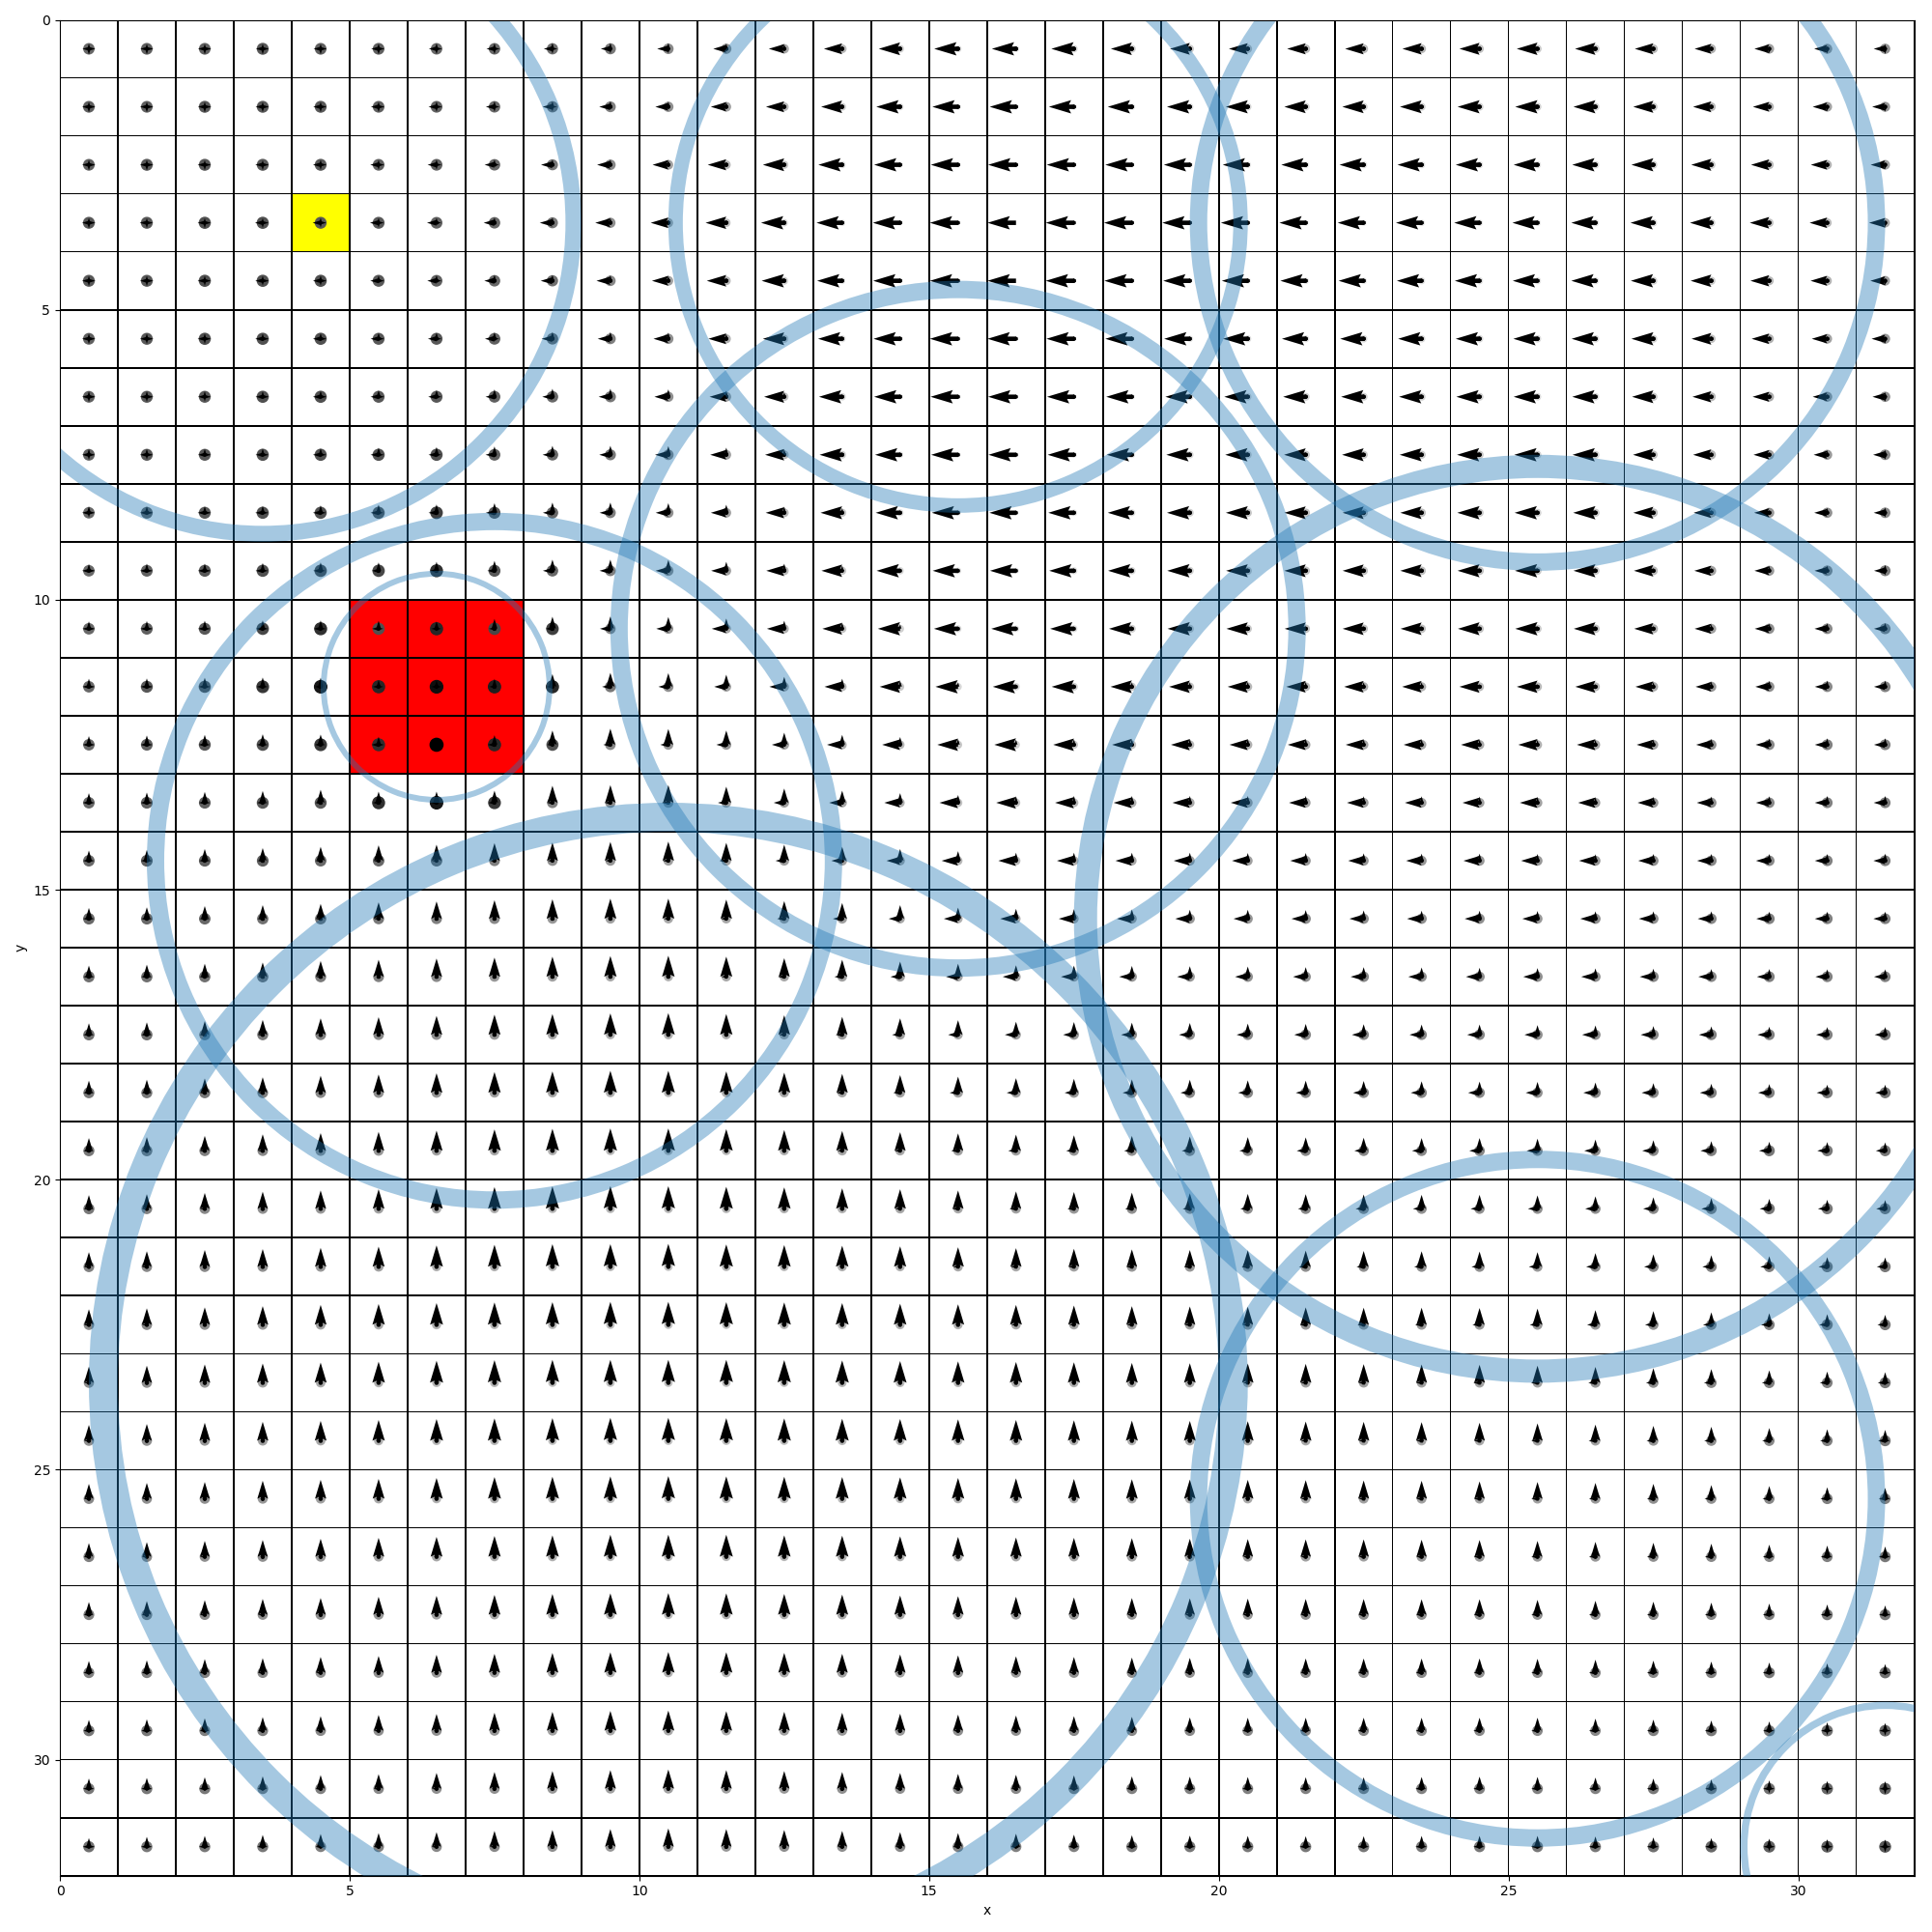
\includegraphics[width=\textwidth]{large_grid_inferred_policy}
				\caption{Inferred policy of \agent{2} in a single agent environment given visitation count (Fig. \ref{fig:large_grid_visit_count}) in a single agent environment. Grid size is 32-by-32. Arrow sizes are proportional to probability of taking the action in each direction.}
				\label{fig:large_grid_inferred_policy}
			\end{minipage}
		}
	\end{center}
\end{figure}


\begin{figure}[H]
	\begin{center}
		\fbox{
			\begin{minipage}{1\textwidth}
				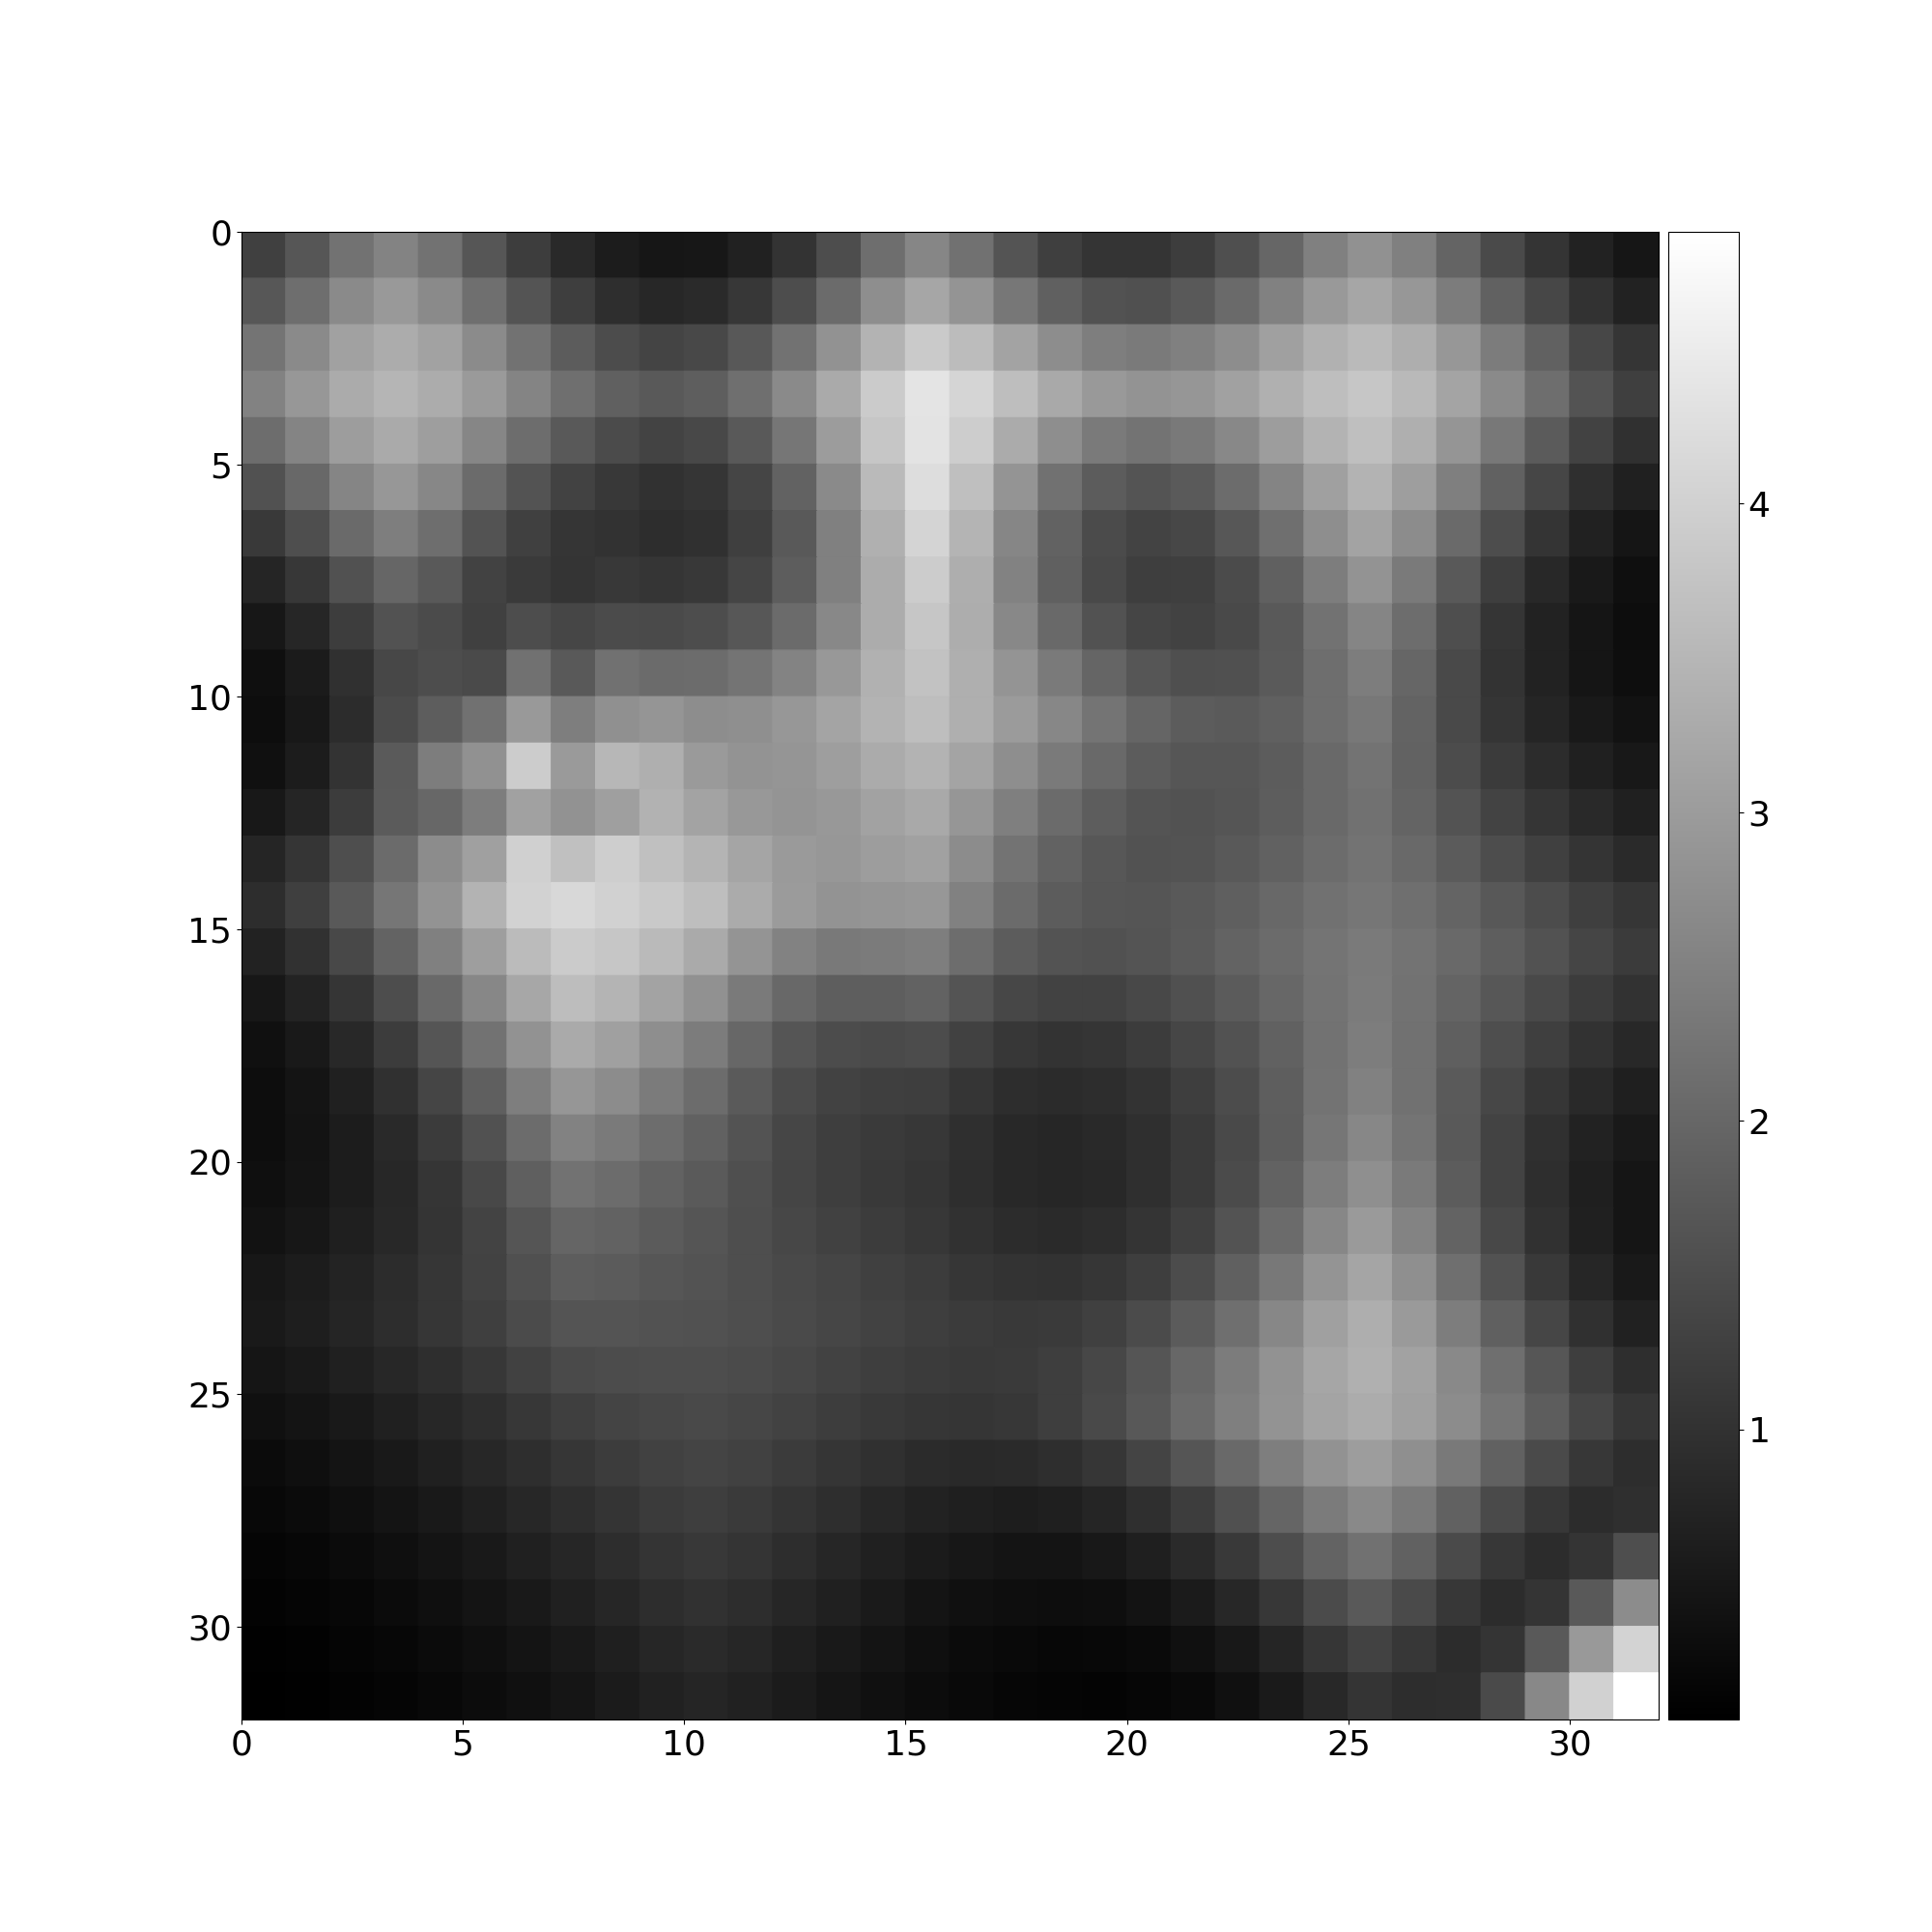
\includegraphics[width=\textwidth]{large_grid_omega}
				\caption{The numerator of Eq. \ref{eq:active_initial_set}, $\sum_{a_2} \Omega(s,a_2)$, is proportional to the probability of initial state being selected after inference results in Fig. \ref{fig:large_grid_inferred_policy}. This heatmap is an alternative visualization of the 3D bar-plot like Fig. \ref{fig:single_agent_uncertainty_surface}}
				\label{fig:large_grid_omega}
			\end{minipage}
		}
	\end{center}
\end{figure}

\begin{figure}[H]
	\begin{center}
		\fbox{
			\begin{minipage}{1\textwidth}
				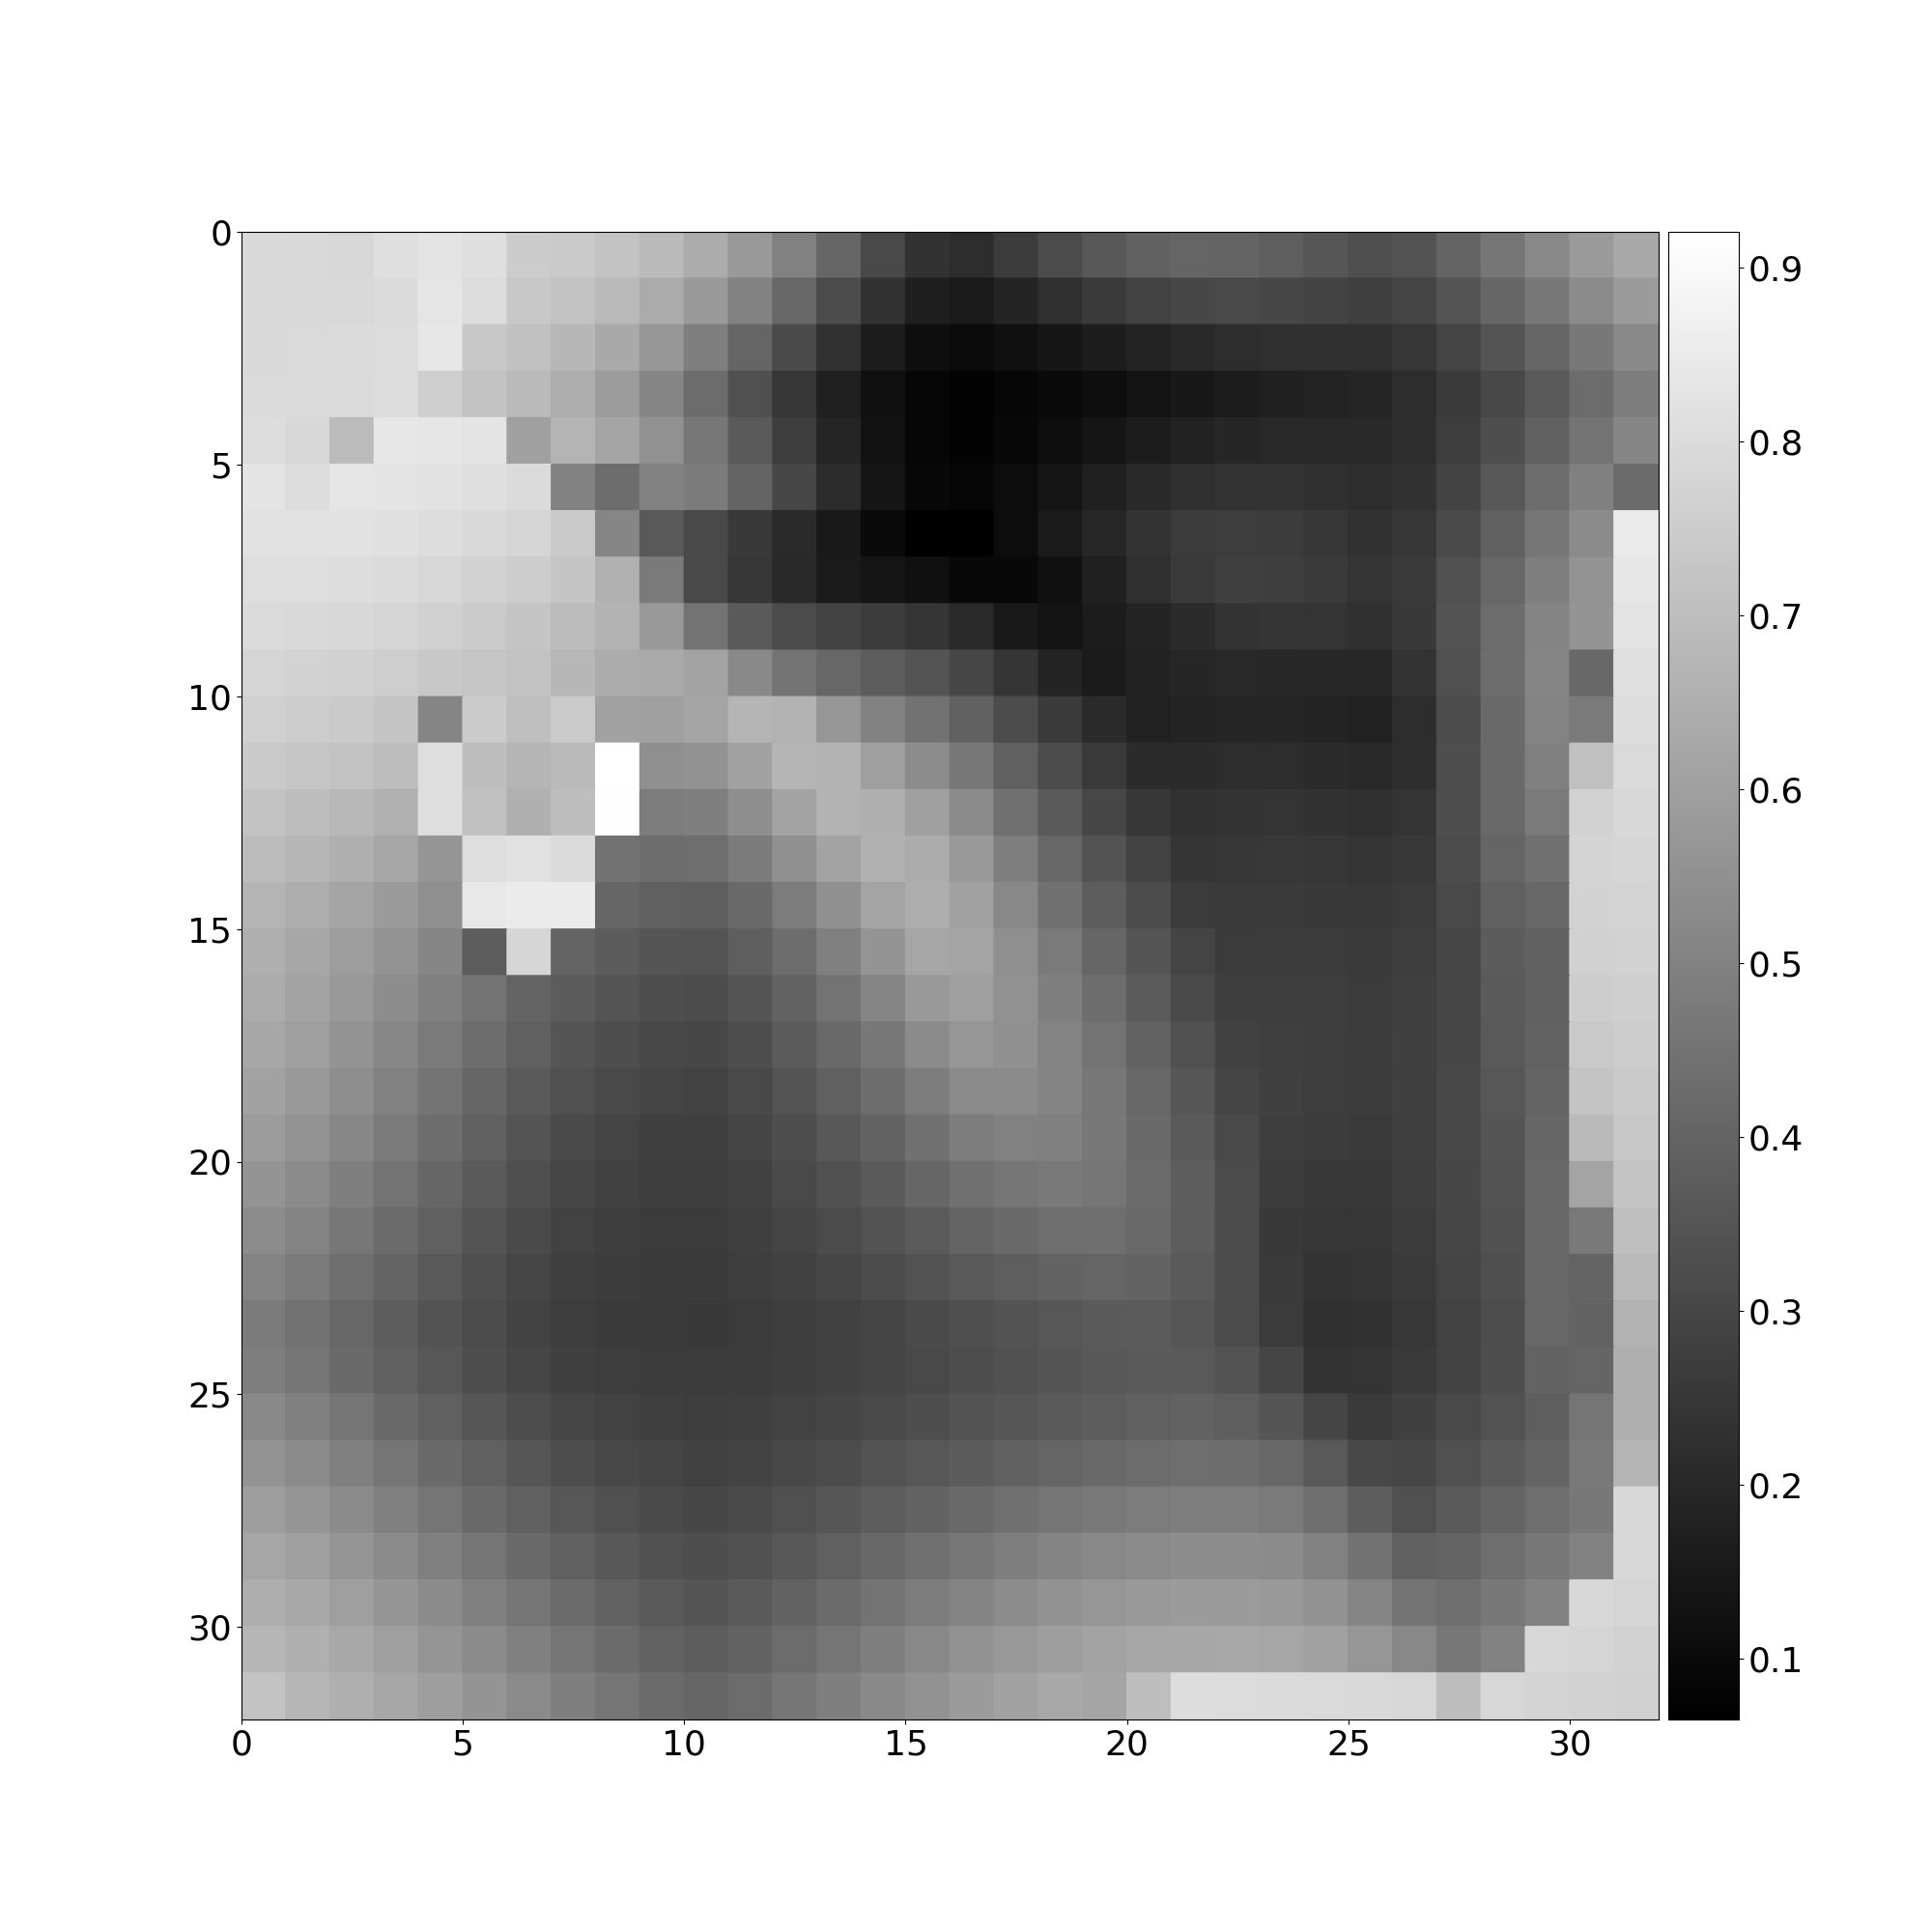
\includegraphics[width=\textwidth]{large_grid_error_magnitude}
				\caption{The true error, \OneNorm{\policy{2},\estimate{\policy{}}_2}, after inference results in Fig. \ref{fig:large_grid_inferred_policy}}
				\label{fig:large_grid_error}
			\end{minipage}
		}
	\end{center}
\end{figure}
